\documentclass[parskip=full]{scrartcl}
\usepackage[utf8]{inputenc} % use utf8 file encoding for TeX sources
\usepackage[T1]{fontenc}    % avoid garbled Unicode text in pdf
\usepackage[german]{babel}  % german hyphenation, quotes, etc
\usepackage{hyperref}       % detailed hyperlink/pdf configuration
\hypersetup{                % ‘texdoc hyperref‘ for options
	pdftitle={Bericht},%
	bookmarks=true,%
}
\usepackage{graphicx}       % provides commands for including figures
\usepackage{csquotes}       % provides \enquote{} macro for "quotes"
\usepackage{scrpage2}
\usepackage{caption}
\usepackage{enumitem}
\pagestyle{scrheadings}
\usepackage{float}

%\clearscrheadfoot
\ohead{BPTI: Gruppe 03=\{Niklas Metz, Felix Bachmann\}, Bericht, WS 2017/18}
\title{BPTI: Bomberman in VHDL}

\begin{document}
	\maketitle
	\section{Beschreibung der Entities}
		\subsection{Bomberman}
		
		\subsection{Game\_mechanic}
		
		\subsection{Game\_state}
		
		\subsection{Player}
		
		\subsection{Movement}
		
		\subsection{Mov\_clk}
		
		\subsection{Bomb}
		
		\subsection{Pixel\_gen}
		
		\subsection{RGB\_assign}
		
		\subsection{Board\_sprites}
		
		\subsection{Player\_sprites}
		
		\subsection{sync\_gen\_ent}
			Die Entity sync\_gen\_ent wird strukturell beschrieben durch die Unterkomponenten hsync und vsync. In dieser Entity werden die Signale für den VGA-Controller generiert (also hsync und vsync). Desweiteren werden zum Setzen der Pixel die aktuelle row und column ausgegeben.
			An dieser Stelle sei auf das VGA-Übungsblatt und den Bericht darüber verwiesen. Wir haben unsere Lösung von dem Übungsblatt für das Projekt übernommen und im Laufe des Projekts nichts an der Entity inklusive Unterkomponenten gerändert.
			\begin{figure}
				\centering
				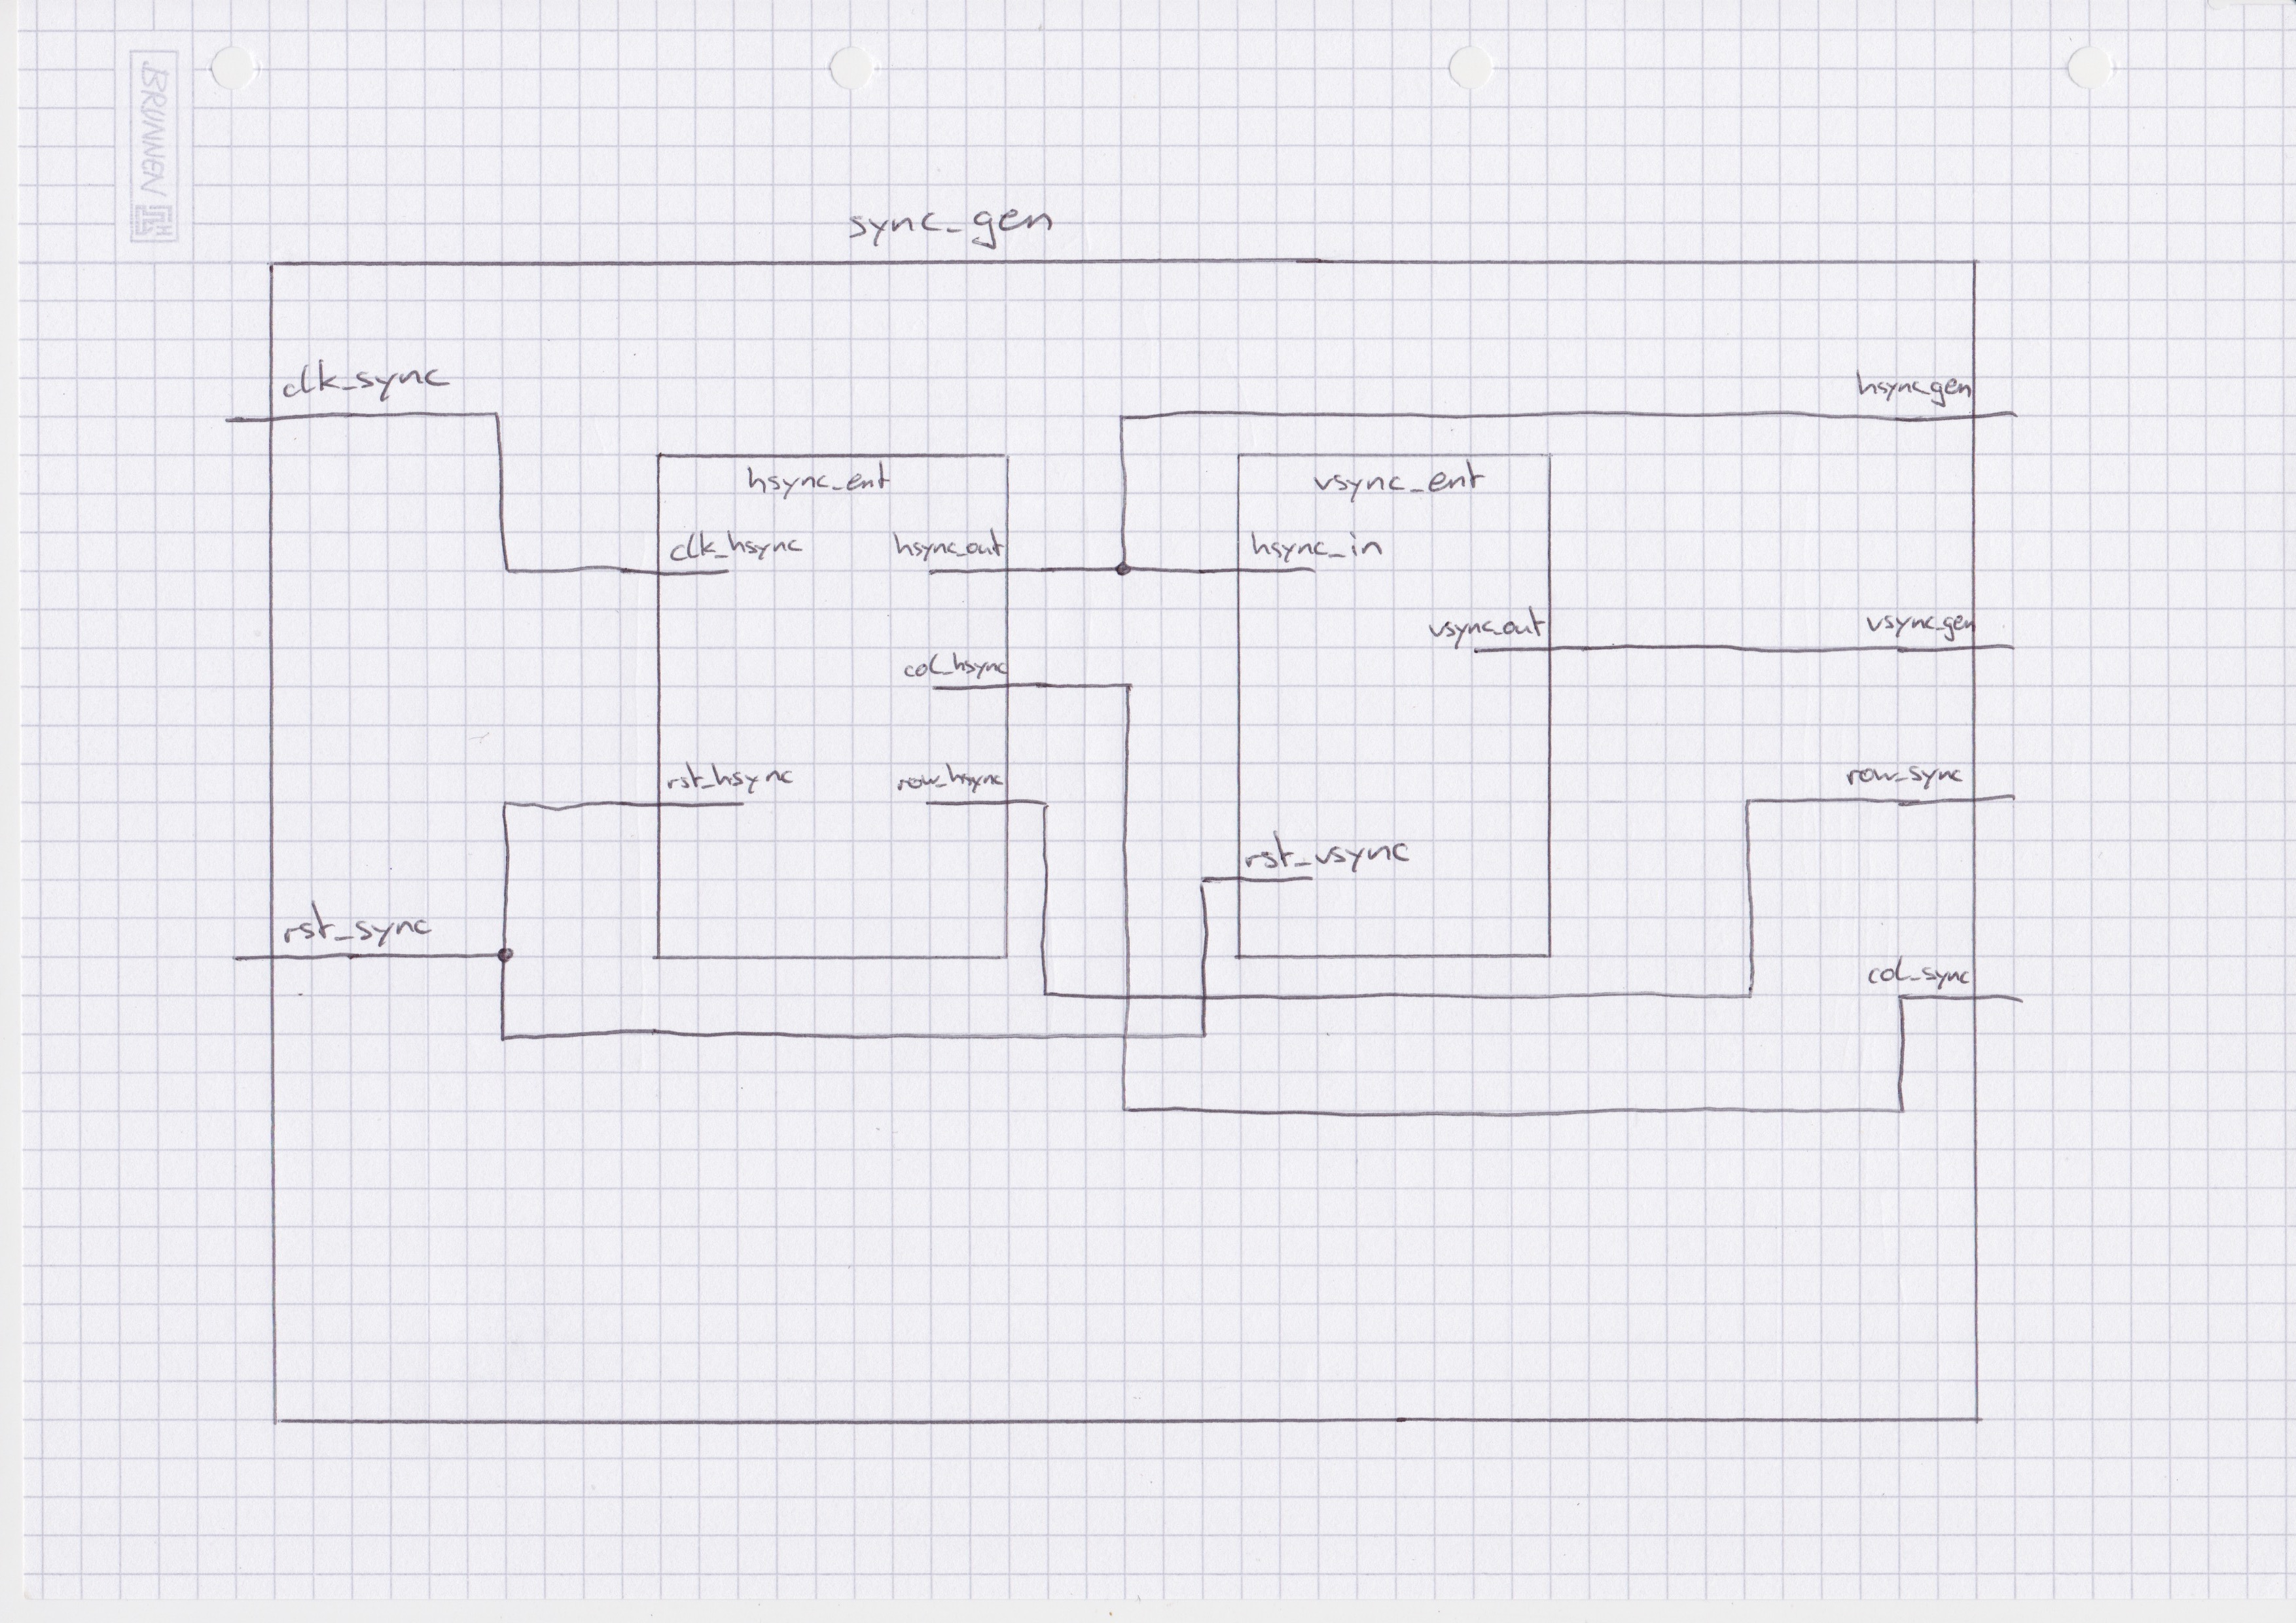
\includegraphics[scale=0.1]{./bilder/Sync_gen.jpeg}
			\end{figure}
		
	\section{Java Dateien}
		\subsection{Main.java}
		
	\section{Probleme}
		\subsection{Bomberman}
		
		\subsection{Game\_mechanic}
		
		\subsection{Game\_state}
		
		\subsection{Player}
		
		\subsection{Movement}
		
		\subsection{Mov\_clk}
		
		\subsection{Bomb}
		
		\subsection{Pixel\_gen}
		
		\subsection{RGB\_assign}
		
		\subsection{Board\_sprites}
		
		\subsection{Player\_sprites}
		
		\subsection{sync\_gen\_ent}
			Ein Problem, das schon bei der Lösung des Übungsblatts aufgetaucht ist, hat sich auch durch das Projekt gezogen.
			Die VGA-Ausgabe funktioniert nicht an allen Monitoren ordnungsgemäß (flackern). An unserem Test-Monitor hat die VGA-Ausgabe nach einigen Einstellungen jedoch funktioniert.
\end{document}